\section{CR Alternativi: kCTF}\label{cr-alternativi-kctf}

kCTF\footnote{\label{fn:ref_2}https://google.github.io/kctf/} e' una piattaforma
sviluppata da Google, basata su \emph{Kubernetes} e \emph{nsjail}.

\begin{quote}
\emph{Kubernetes}: e' un sistema open source per automatizzare il
deploy, scalare e gestire applicazioni containerizzate.\footnote{\label{fn:ref_3}https://kubernetes.io/}
\end{quote}

\begin{quote}
\emph{NSJail}: ossia, NameSpace Jail, e' un tool Linux per isolare i
processi utilizzando varie feature del Kernel Linux come: namespaces,
resource limits, seccomp-bpf syscall filters. L'obiettivo di NSJail e'
quello di creare un'ambiente sicuro e isolato per eseguire le
applicazioni. \footnote{\label{fn:ref_4}https://github.com/google/nsjail/}
\end{quote}


\begin{figure}[htbp]
  \centering
  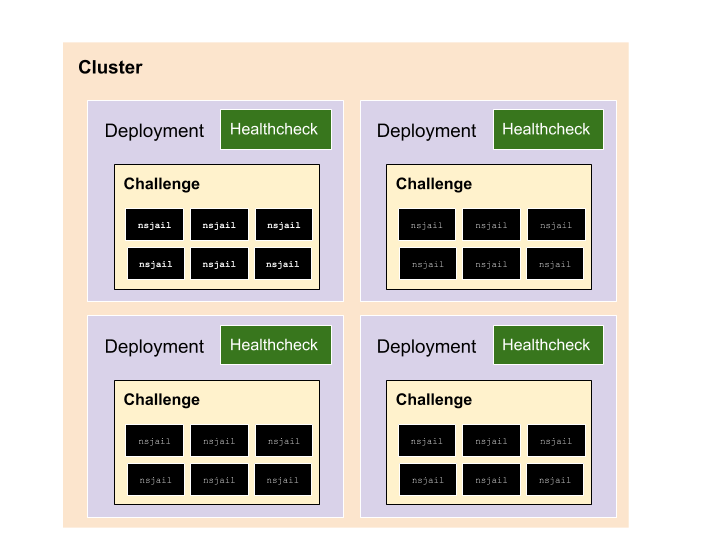
\includegraphics[width=0.92\linewidth,height=0.7\textheight,keepaspectratio]{src/images/kctf-architecture.png}
  \caption{Kctf Architecture}
  \label{fig:kctf-architecture}
\end{figure}


Facendo riferimento all'immagine sopra, l'architettura di kCTF prevede:

\begin{itemize}
\tightlist
\item
  Un \textbf{cluster}, che contiene un'insieme di challenge
\item
  Dei \textbf{deployment}, ognuno contiene due container (o meglio, un
  Pod che instanzia 2 container):

  \begin{itemize}
  \tightlist
  \item
    un container \passthrough{\lstinline!healthcheck!}: usato per
    determinare lo stato di salute dei servizi
  \item
    un container \passthrough{\lstinline!challenge!}: contiene i servizi
    su cui lavora lo sfidante.
  \end{itemize}
\end{itemize}

\begin{quote}
\textbf{Pod}: in Kubernetes, e' la piu piccola unita che Kubernetes puo'
eseguire. Un Pod, rappresenta uno o piu container in esecuzione su un
singolo nodo.\footnote{\label{fn:ref_5}https://www.k8s.guide/workloads/pods-deployments/}
\end{quote}

\begin{quote}
\textbf{Deployment}: in Kubernetes, un deployment e' un template che
specifica come creare i container. I template guidano la creazione di
\textbf{Pods} e la gestione sicura del ciclo di vita di un Pod, in
particolare la gestione dei ReplicaSet.\footref{fn:ref_5}
\end{quote}

NSJail viene avviato su ogni container
\passthrough{\lstinline!challenge!}, ed e' configurato per ascoltare su
una porta TCP nota. Ad ogni connessione TCP in arrivo, NSJail esegue un
fork restituendo allo sfidante un'ambiente separato (rispetto agli altri
sfidanti) su cui lavorare. L'obiettivo di questa architettura e' di
poter riutilizzare lo stesso container per piu sfidanti.

L'isolamento fornito da NSJail, si ottiene combinando varie tecniche:

\begin{itemize}
\tightlist
\item
  Creazione di nuovi namespace: l'ambiente fornito, esegue su un nuovo
  namespace, separando logicamente le risorse accessibili.
\item
  Filtraggio delle chiamate di sistema tramite
  \passthrough{\lstinline!seccomp-bpf!}: questo sottosistema permette di
  uccidere i processi nell'ambiente se vengono eseguite chiamate di
  sistema vietate.
\item
  Accounting e limitazione delle risorse con
  \passthrough{\lstinline!cgroup!}: questo sottosistema permette di
  monitorare e limitare le risorse utilizzabili nel nuovo ambiente.
\end{itemize}

NsJail puo' essere configurato in modo che ogni ambiente isolato, abbia
a disposizione un'filesystem temporaneo che risiede in RAM, mentre il
filesystem originale e' accessibile dall'ambiente sandbox in sola
lettura. Questa configurazione e' necessaria poiche altrimenti gli
sfidanti modificherebbero tutti lo stesso filesystem.

Un'altra configurazione di NSJail e' la seguente: che e' ideale per le
challenge di tipo \passthrough{\lstinline!pwn!} (trovare e sfruttare
vulnerabilita in file binari):

\begin{lstlisting}
[...]
mount: [
  {
    src: "/chroot"
    dst: "/"
    is_bind: true
  },
  {
    dst: "/tmp"
    fstype: "tmpfs"
    rw: true
  },
  {
    dst: "/proc"
    fstype: "proc"
    rw: true
  },
  {
    src: "/etc/resolv.conf"
    dst: "/etc/resolv.conf"
    is_bind: true
  }
]
\end{lstlisting}

\begin{enumerate}
\def\labelenumi{\arabic{enumi}.}
\tightlist
\item
  La cartella \passthrough{\lstinline!/chroot!} che risiede nel
  container, diventa la radice nel nuovo ambiente.
\item
  Viene creato un nuovo \passthrough{\lstinline!tmpfs!}, in
  \passthrough{\lstinline!/tmp!}
\item
  Viene importata la configurazione DNS da
  \passthrough{\lstinline!/etc/resolv.conf!} dentro la nuova radice.
\end{enumerate}

Tutta via, l'uso di NsJail per separare gli ambienti dei partecipanti,
rende difficoltosa l'implementazione di challenge in cui si vuole dare
la liberta ai partecipanti di installare pacchetti dentro al container,
oppure di modificare file di configurazione che risiedono per esempio in
\passthrough{\lstinline!/etc!} e di modificare direttamente servizi in
esecuzione sul container. \footnote{\label{fn:ref_6}https://github.com/google/kctf/blob/v1/docs/security-threat-model.md}

Queste limitazioni ci sono perche NsJail nell'ambiente sandbox non
fornisce una propria istanza di \passthrough{\lstinline!systemd!} (o un
qualsiasi gestore di servizi) e neanche l'infrastruttura necessaria per
eseguiure comandi come \passthrough{\lstinline!apt!}.

NsJail porta con se altri problemi:

\begin{itemize}
\tightlist
\item
  Se dovesse cadere la connessione TCP allora tutto il contenuto del
  filesytem in RAM andrebbe perso.
\item
  L'uso di \passthrough{\lstinline!seccomp!} per filtrare le chiamate di
  sistema potrebbe impedire l'esecuzione di alcuni programmi
  fondamentali per la challenge.
\end{itemize}

Dunque kCTF potrebbe essere utilizzato per implementare un Cyber Range
difensivo ma con varie limitazioni e problemi da raggirare.

L'approccio di kCTF e' completamente all'opposto di quanto fatto in
BlueAgent ed in altri Cyber Range. BlueAgent si occupa di gestire piu
container per ogni team, mentre kCTF assegna un container per tutti i
team da dividre usando ambienti separati con NsJail.

Di seguito sono riportate le principali differenze tra kCTF ed NsJail:

\begin{longtable}[]{@{}
  >{\raggedright\arraybackslash}p{(\linewidth - 4\tabcolsep) * \real{0.3333}}
  >{\raggedright\arraybackslash}p{(\linewidth - 4\tabcolsep) * \real{0.3333}}
  >{\raggedright\arraybackslash}p{(\linewidth - 4\tabcolsep) * \real{0.3333}}@{}}
\toprule\noalign{}
\begin{minipage}[b]{\linewidth}\raggedright
Caratteristica
\end{minipage} & \begin{minipage}[b]{\linewidth}\raggedright
kCTF
\end{minipage} & \begin{minipage}[b]{\linewidth}\raggedright
BlueAgent
\end{minipage} \\
\midrule\noalign{}
\endhead
\bottomrule\noalign{}
\endlastfoot
\textbf{Virtualizzazione} & Container applicativi e sandbox di processo
(NSJail) & Container di sistema, ognuno con un suo gestore di
servizi. \\
\textbf{Infrastruttura} & Cluster distribuito Kubernetes & Singolo nodo
host \\
\textbf{Ambiente Dedicato } & Un solo container condiviso tra sfidanti &
Container di sistema dedicati e separati per ciascun team \\
\textbf{Persistenza} & Filesystem effimero in RAM
(\passthrough{\lstinline!tmpfs!}) & Persistente su disco \\
\textbf{Provisioning} & Istantaneo (consiste nel fork con NsJail) &
Rapido (consiste nel deploy di uno o piu container) \\
\end{longtable}
